\begin{figure}[!htb]
\centering
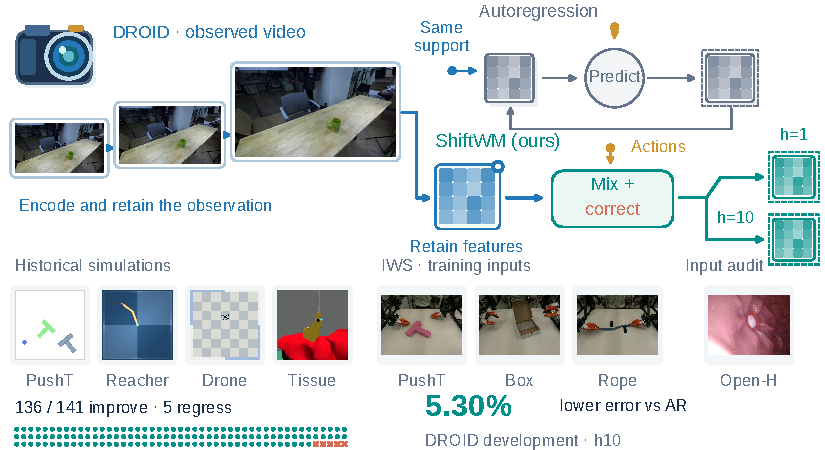
\includegraphics[width=\linewidth]{generated/editorial/teaser_camera_story.pdf}
\caption[Forecast from retained observations.]{\textbf{Forecast from retained observations.} Three recorded DROID frames supply fixed support features and the last-observed reference $Z_0$; the palette compresses this interface (Figure~\ref{fig:editorial-spatial-method}). ShiftWM conditions every query on this support and supplied causal commands; autoregression rolls its own predictions into the next feature history, keeping inferred context fixed. Two schematic endpoints illustrate feature forecasts, not generated RGB; the camera is illustrative. Historical simulations use distinct models; IWS training is ongoing; Open-H is a physical-phantom input audit. All 141 DROID development episodes remain visible. The 5.30\% reduction compares population mean native, training-standardized $h=10$ feature MSE with matched autoregression; uncertainty: Figure~\ref{fig:editorial-spatial}. Images: DROID/Open-H (CC BY 4.0); IWS \citep{zhang2026rlawm}.}
\label{fig:editorial-teaser}
\end{figure}
